\chapter{Versuchen}
\label{chap:Versuchen}

\section{Untersuchungsplattform}
\label{sec:Untersuchungsplattform}
Unsere Untersuchung wurde durchgeführt auf dem Plattform wie unter:

\begin{table}[htbp]
\begin{center}
\begin{tabular}{ l | l }
	Hardwaresystem 	& ODROID-XU3 Lab Environment(mit ARM Cortex-A7\\
					& 1.4Ghz und Cortex-A15 2.0Ghz big.LITTLE\\
					& architecture jeweils 4 kerne)\\ \hline
	Betribssystem 	& Ubuntu 15.10 mit ssh Zugriff und shared storage\\
					& durch NFS server\\ \hline
	Test-Benchmark 	& NAS Parallel Benchmarks\\ \hline
	Tasks 			& LU Dekomposition und Gauß'sche Elimination(LU)\\ 
					& und konjugierender Gradient(CG)\\ \hline
	Task-Maßstab	& siehe Tablett \ref{tab:Task-Massstab}\\ \hline
	Implementationssprache 	& Java mit Fortran zusammenarbeiten\\ \hline
	Implementationsmethode 	& OpenMP und MPI(Message Passing Interface)\\ \hline
	Messungsgeräte & ODROID Smart Power Device 
\end{tabular}
\end{center}
\label{tab:Untersuchungsplattform}
\caption{Untersuchungsplattform}
\end{table}

\begin{table}[htbp]
\begin{center}
\begin{tabular}{l|l|l|l}
	&			&Class A 	&Class B\\ \hline
CG 	&Size		&14000		&75000\\
	&Iteration	&15			&75\\ \hline
LU 	&Size		&64x64x64	&102x102x102\\
	&Iteration	&250		&250\\
\end{tabular}
\end{center}
\label{tab:Task-Massstab}
\caption{Task-Maßstab}
\end{table}

\section{Energiebedarf-relevante Aspekte}
\label{sec:Energiebedarf-relevante Aspekte}

\subsection{Energiebedarf und Architektur}
\label{subsec:Energiebedarf und Architektur}

\begin{figure}[ht]
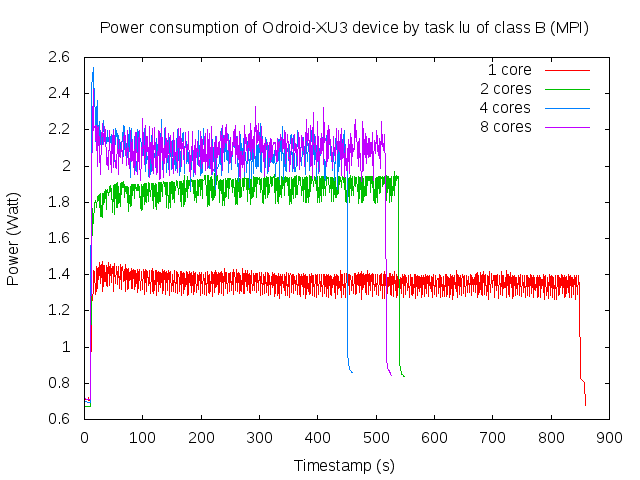
\includegraphics[width=\textwidth]{cores_power}
\caption[Leistung und Kernenutzung]{Leistung und Kernenutzung}
\label{fig:Leistung und Kernenutzung}
\end{figure}

\begin{figure}[ht]
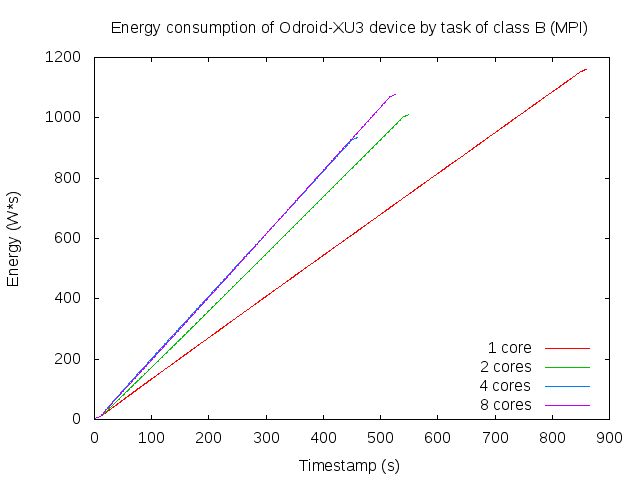
\includegraphics[width=\textwidth]{cores_energy}
\caption[Energiebedarf und Kernenutzung]{Energiebedarf und Kernenutzung}
\label{fig:Energiebedarf und Kernenutzung}
\end{figure}

\begin{figure}[ht]
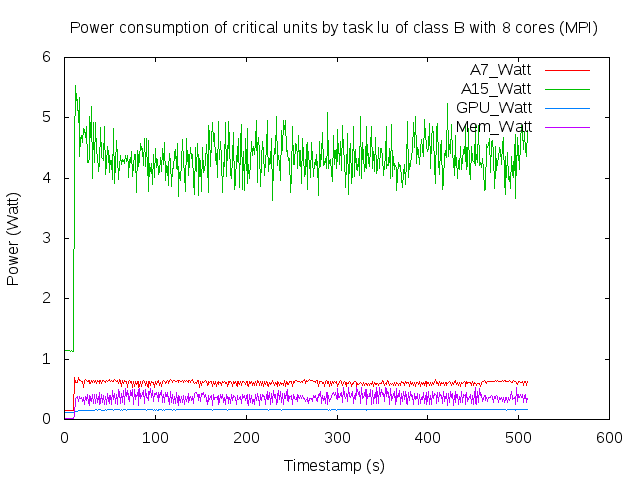
\includegraphics[width=\textwidth]{units_power}
\caption[Leistung kritischer Teilen]{Leistung kritischer Teilen}
\label{fig:Leistung kritischer Teilen}
\end{figure}

Die Abbildung \ref{fig:Leistung und Kernenutzung} und sein Integral Abbildung \ref{fig:Energiebedarf und Kernenutzung} stell dar, Leistung und Energiebedarf von ganze ODROID-XU3 Computer. Die Konfiguration lautet, das Task von LU und mit Klasse B ist.

\subsection{Energiebedarf und Tasks}
\label{subsec:Energiebedarf und Tasks}

\begin{figure}[ht]
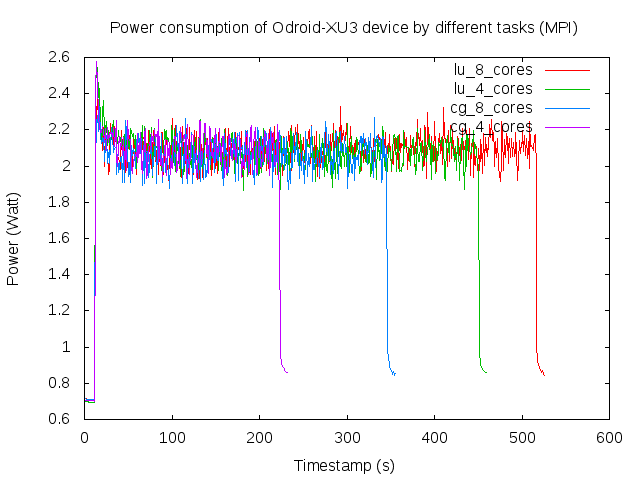
\includegraphics[width=\textwidth]{tasks_power}
\caption[Leistung und Tasks]{Leistung und Tasks}
\label{fig:Leistung und Tasks}
\end{figure}

\begin{figure}[ht]
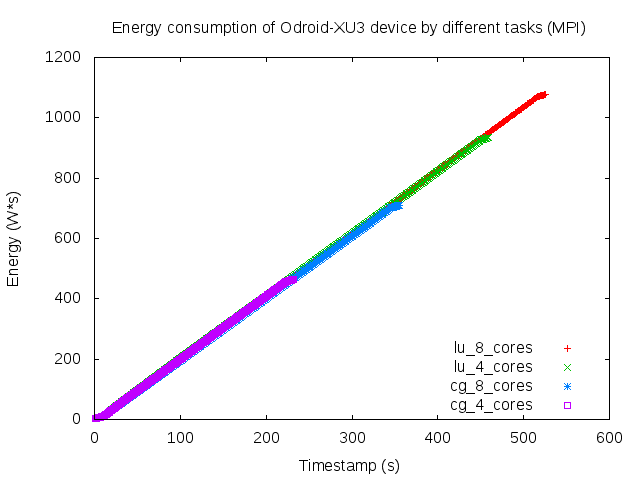
\includegraphics[width=\textwidth]{tasks_energy}
\caption[Energiebedarf und Tasks]{Energiebedarf und Tasks}
\label{fig:Energiebedarf und Tasks}
\end{figure}

Die Abbildung \ref{fig:Leistung und Tasks} und ihre Integral \ref{fig:Energiebedarf und Tasks}, zeigen die Beziehung zwischen Leistung zusammen mit Energiebedarf und verschidene Tasks.

\subsection{Energybedarf und Maßstab von Tasks}
\label{subsec:Energybedarf und Massstab von Tasks}

\begin{figure}[ht]
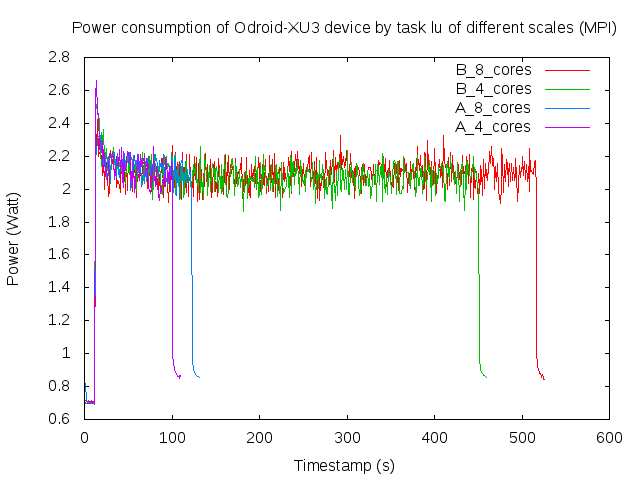
\includegraphics[width=\textwidth]{scales_power}
\caption[Leistung und Maßstab von Tasks]{Leistung und Maßstab von Tasks}
\label{fig:Leistung und Massstab von Tasks}
\end{figure}

\begin{figure}[ht]
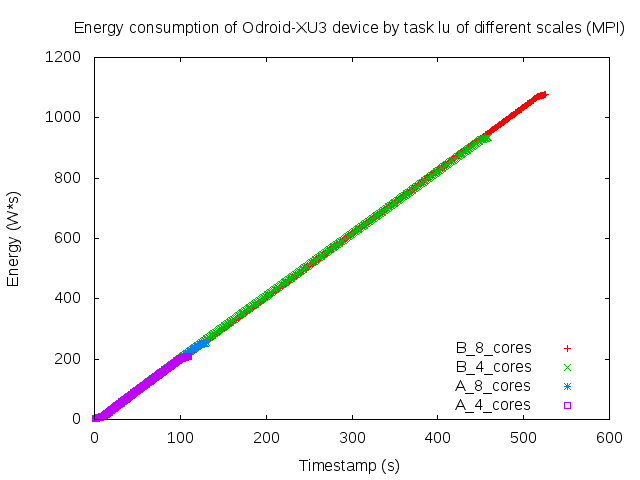
\includegraphics[width=\textwidth]{scales_energy}
\caption[Energiebedarf und Maßstab von Tasks]{Energiebedarf und Maßstab von Tasks}
\label{fig:Energiebedarf und Massstab von Tasks}
\end{figure}

Die Abbildungen \ref{fig:Leistung und Massstab von Tasks} und \ref{fig:Energiebedarf und Massstab von Tasks} zeigen die Beziehung zwischen Leistung zusammen mit Energiebedarf von ganze Systeme und Massstab von Tasks.

\subsection{Energy bedarf und Implementationsmethode}
\label{subsec:Energy bedarf und Implementationsmethode}

\begin{figure}[ht]
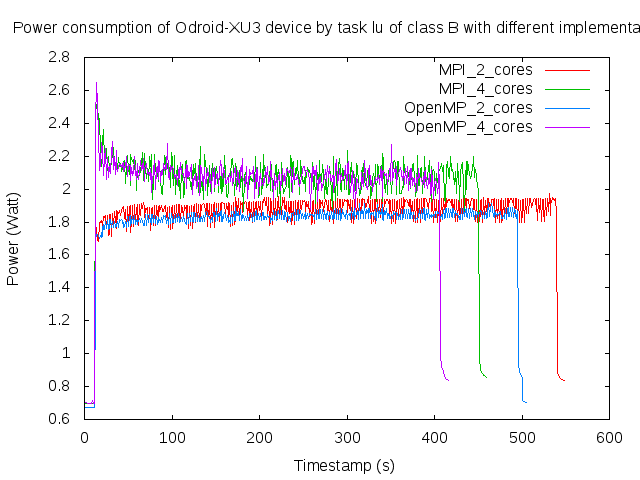
\includegraphics[width=\textwidth]{implementations_power}
\caption[Leistung und Implementationsmethode]{Leistung und Implementationsmethode}
\label{fig:Leistung und Implementationsmethode}
\end{figure}

\begin{figure}[ht]
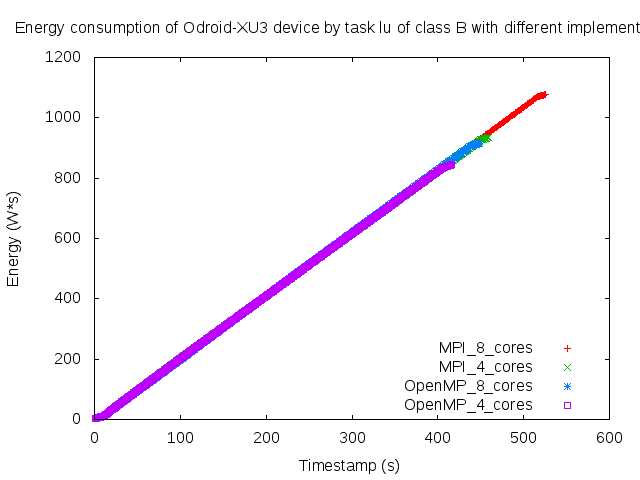
\includegraphics[width=\textwidth]{implementations_energy}
\caption[Energiebedarf und Implementationsmethode]{Energiebedarf und Implementationsmethode}
\label{fig:Energiebedarf und Implementationsmethode}
\end{figure}

Die Abbildungen \ref{fig:Leistung und Implementationsmethode} und \ref{fig:Energiebedarf und Implementationsmethode} stellen her, wie sich die Leistung und Energiebedarf wegen des Implementationsnterschieds veränden.
